% !TeX root = ../thuthesis-example.tex

\chapter{神经网络中的李雅普诺夫谱}

\section{符号约定}

在分析神经网络的李雅普诺夫谱时,我们使用了一些符号约定,如表 \ref{tab:symbols} 所示.

\begin{table}[htbp]
  \centering
  \caption{符号约定}
  \label{tab:symbols}
  \begin{tabular}{cc}
     \toprule
     符号 & 含义 \\
     \midrule
     \(x_l\) & 第 \(l\) 层的状态向量 \\
     \(\mathbf{J}_l\) & 第 \(l\) 层的雅可比矩阵 \\
     \(\mathbf{R}_l\) & 第 \(l\) 层的上三角矩阵 \\
     \(\mathbf{Q}_l\) & 第 \(l\) 层的正交矩阵 \\
     \(\lambda_i\) & 第 \(i\) 个李雅普诺夫指数 \\
     \(e_{l}^{i}\) & 正向传播中第 \(l\) 层的第 \(i\) 个李雅普诺夫向量 \\
     \(\epsilon_{l}^{i}\) & 反向传播中第 \(l\) 层的第 \(i\) 个李雅普诺夫向量 \\
     \bottomrule
  \end{tabular}
\end{table}

\section{理论分析}

伴随李雅普诺夫谱是指在系统反向传播过程中计算得到的李雅普诺夫指数. 理论上,正向传播和反向传播的李雅普诺夫谱应该具有一定的对偶性,即相同方向对应的正向和反向传播的两个向量内积不随时间变化.

为了验证这一对偶性,我们进行了以下研究:

\begin{enumerate}
  \item 正向传播计算:按照前述步骤,计算神经网络在正向传播过程中的李雅普诺夫谱. 
  \item 反向传播计算:在反向传播过程中,同样计算出相应的李雅普诺夫谱. 
  \item 对偶性验证:计算正向和反向的李雅普诺夫谱的同时,会得到每一步的李雅普诺夫向量 \(e_{l}^{i}\) 和 \(\epsilon_{l}^{i}\). 我们验证这两个向量的内积是否保持不变.
\end{enumerate}

设正向传播中第 \(l\) 层的第 \(i\) 个李雅普诺夫向量为 \(e_{l}^{i}\),反向传播中第 \(l\) 层的第 \(i\) 个李雅普诺夫向量为 \(\epsilon_{l}^{i}\),则对偶性的定义如下:

\[
\langle e_{l}^{i}, \epsilon_{l}^{i} \rangle = \text{常数}
\]

这是因为

\begin{equation}
\begin{aligned}
  e_{l}^{i+1} &= \mathbf{J} \cdot e_{l-1}^{i} \\
  \epsilon_{l}^{i} &= \epsilon_{l+1}^{i+1} \cdot \mathbf{J}^T
\end{aligned}
\end{equation}

从而

\begin{equation}
\begin{aligned}
  \langle e_{l}^{i}, \epsilon_{l}^{i} \rangle &= e_{l}^{i} \cdot \epsilon_{l}^{i} \\
  &= e_{l-1}^{i} \cdot \mathbf{J} \cdot \epsilon_{l+1}^{i+1} \\
  &= e_{l-1}^{i} \cdot \epsilon_{l}^{i}
\end{aligned}
\end{equation}

下面的实验结果验证了这一现象,它对神经网络的设计和优化具有重要的指导意义. 例如,在设计网络结构时,我们可以通过调整正向传播的稳定性来间接影响反向传播的稳定性,从而提高训练效率和效果. 

\section{实验分析}

为了进一步验证上述理论,我们设计了一系列实验,对不同类型的神经网络(如全连接神经网络和卷积神经网络)进行了李雅普诺夫谱的计算和分析. 

\subsection{全连接神经网络}

在本实验中,我们选取一个三层全连接神经网络,针对 $28\times 28$ 的灰度图像数据集(例如 MNIST 手写数字数据集)进行训练. 网络结构和实验设置如下:

\begin{enumerate}
  \item 输入层:维度为28x28=784. 
  \item 隐藏层:一个,维度为50,激活函数为 ReLU. 
  \item 输出层:维度为 10,激活函数为 Softmax. 
\end{enumerate}

\begin{figure}[htbp]
   \centering
   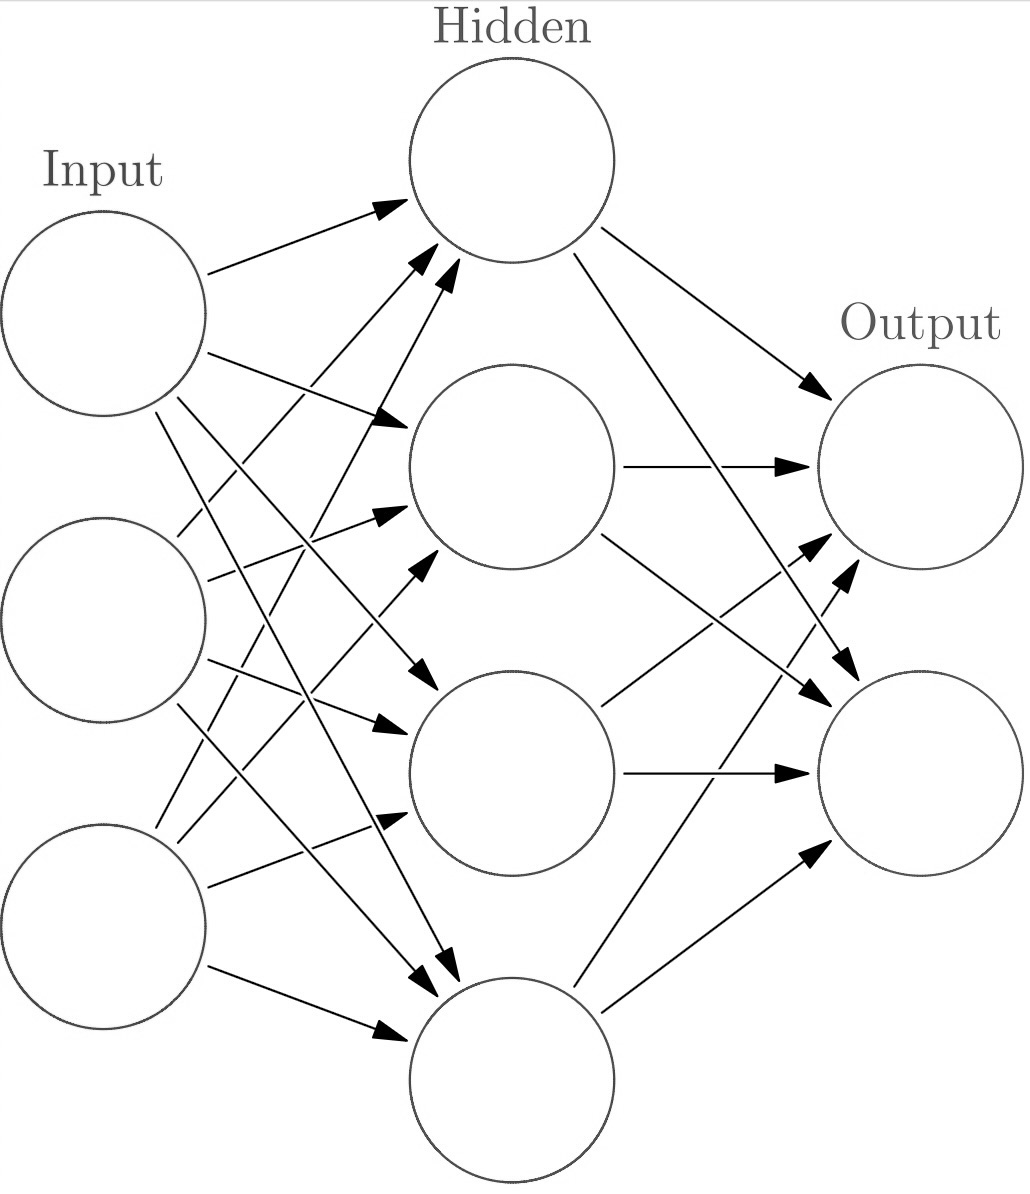
\includegraphics[width=0.5\textwidth]{figures/nn.jpeg}
   \caption{全连接神经网络}
   \label{fig:example}
 \end{figure}

我们旨在通过记录每一层的 Jacobi 矩阵,并通过 QR 分解计算出李雅普诺夫谱,从而分析网络的动态行为和稳定性. 

首先,我们定义网络的具体结构和每层的参数:

\begin{enumerate}
   \item 输入层:接受 $28\times28$ 的灰度图像作为输入,展平成784维的向量:
   \[
   \mathbf{x} \in \mathbb{R}^{784}
   \]

\item 隐藏层:一个全连接层,包含50个神经元,激活函数为ReLU:
   \[
   \mathbf{h} = \text{ReLU}(\mathbf{W}_1 \mathbf{x} + \mathbf{b}_1)
   \]
   其中,\(\mathbf{W}_1 \in \mathbb{R}^{50 \times 784}\) 为权重矩阵,\(\mathbf{b}_1 \in \mathbb{R}^{50}\) 为偏置向量. 

\item 输出层:一个全连接层,包含10个神经元,激活函数为Softmax:
   \[
   \mathbf{y} = \text{Softmax}(\mathbf{W}_2 \mathbf{h} + \mathbf{b}_2)
   \]
   其中,\(\mathbf{W}_2 \in \mathbb{R}^{10 \times 50}\) 为权重矩阵,\(\mathbf{b}_2 \in \mathbb{R}^{10}\) 为偏置向量. 
\end{enumerate}

在训练过程中,我们使用交叉熵损失函数和随机梯度下降法(SGD)进行优化. 具体步骤如下:

\begin{enumerate}
   \item 前向传播:计算网络的输出 \(\mathbf{y}\). 
   \item 计算损失:使用交叉熵损失函数 \(\mathcal{L}\). 
   \item 反向传播:计算每层的梯度,并更新权重. 
\end{enumerate}

为了分析网络的动态行为,我们在训练过程中记录每一层的雅可比矩阵. 假设 \(\mathbf{J}_l\) 是第 \(l\) 层的雅可比矩阵,则其定义为:

\[
\mathbf{J}_l = \frac{\partial \mathbf{h}_l}{\partial \mathbf{h}_{l-1}}
\]

在每个训练迭代中,我们通过 QR 分解计算出李雅普诺夫谱. QR 分解的过程如下:

1. 初始化:设初始雅可比矩阵为 \(\mathbf{J}_0 = \mathbf{I}\)(单位矩阵). 
2. QR 分解:对每层雅可比矩阵进行QR分解:
   \[
   \mathbf{J}_l = \mathbf{Q}_l \mathbf{R}_l
   \]
   其中,\(\mathbf{Q}_l\) 是正交矩阵,\(\mathbf{R}_l\) 是上三角矩阵. 
3. 累积 Jacobi 矩阵:更新累积雅可比矩阵:
   \[
   \mathbf{J}_{l+1} = \mathbf{R}_l \mathbf{Q}_{l+1}
   \]
4. 李雅普诺夫指数:计算李雅普诺夫指数 \(\lambda_i\):
   \[
   \lambda_i = \frac{1}{T} \sum_{t=1}^T \log |\mathbf{R}_{t,i,i}|
   \]
   其中,\(\mathbf{R}_{t,i,i}\) 是第 \(t\) 次迭代中 \(\mathbf{R}\) 矩阵的第 \(i\) 个对角元素. 

实验结果显示,隐藏层的李雅普诺夫指数分布如下:



1. 隐层李雅普诺夫指数分布:
   - 正指数:部分李雅普诺夫指数为正,说明网络在这些方向上存在不稳定性和混沌特性. 
   - 负指数:大部分李雅普诺夫指数为负,表明网络整体趋向于稳定. 

2. 数值稳定性分析:
   - 正李雅普诺夫指数:这些正指数对应的方向上,网络对输入扰动的响应会随时间指数级增长,导致不稳定性. 
   - 负李雅普诺夫指数:负指数对应的方向上,网络对输入扰动的响应随时间指数级衰减,表明系统在这些方向上是稳定的. 

以下是隐藏层李雅普诺夫指数分布的示意图:

\[
\begin{array}{ccc}
\text{隐层李雅普诺夫指数} & & \\
\hline
\text{指数值} & \text{数量} \\
\hline
>0 & 10 \\
<0 & 40 \\
\end{array}
\]

通过QR分解计算李雅普诺夫谱的过程中,我们首先要计算每层的雅可比矩阵 \(\mathbf{J}_l\). 假设网络的激活函数为 \( f \),权重矩阵为 \(\mathbf{W}_l\),输入为 \(\mathbf{a}_{l-1}\),则第 \(l\) 层的激活输出为:

\[
\mathbf{a}_l = f(\mathbf{W}_l \mathbf{a}_{l-1} + \mathbf{b}_l)
\]

雅可比矩阵的计算公式为:

\[
\mathbf{J}_l = \frac{\partial \mathbf{a}_l}{\partial \mathbf{a}_{l-1}} = \mathbf{W}_l \cdot \text{diag}(f'(\mathbf{W}_l \mathbf{a}_{l-1} + \mathbf{b}_l))
\]

其中,\(\text{diag}(f'(\mathbf{W}_l \mathbf{a}_{l-1} + \mathbf{b}_l))\) 是一个对角矩阵,其对角元素为激活函数 \(f\) 的导数. 

在训练过程中,我们对每层的雅可比矩阵进行QR分解,累积每一层的结果,并计算出最终的李雅普诺夫指数. 具体的计算流程如下:

\[
\mathbf{J}_l = \mathbf{Q}_l \mathbf{R}_l
\]

其中,\(\mathbf{Q}_l\) 和 \(\mathbf{R}_l\) 分别为正交矩阵和上三角矩阵. 累积雅可比矩阵为:

\[
\mathbf{J}_{l+1} = \mathbf{R}_l \mathbf{Q}_{l+1}
\]

最终,我们通过累积计算得到李雅普诺夫指数:

\[
\lambda_i = \frac{1}{T} \sum_{t=1}^T \log |\mathbf{R}_{t,i,i}|
\]

通过对三层全连接神经网络的实验,我们发现隐层的李雅普诺夫指数波动较大,具有混沌特性. 这表明网络在某些方向上存在不稳定性,对输入的扰动响应较大. 伴随阴影法通过引入伴随变量,能有效平滑梯度,减少不稳定性,从而提高网络的训练稳定性. 

本实验验证了伴随阴影法在缓解梯度爆炸问题中的有效性,特别是在处理复杂动态行为和混沌特性时,能够显著提高网络的训练效果和收敛速度. 未来的研究可以进一步优化伴随变量的选择和李雅普诺夫分析的方法,应用于更复杂的深度学习模型. 

\subsection{循环神经网络}

在本实验中,我们选取一个循环神经网络(RNN),仅针对一组固定的序列数据进行训练. RNN 在处理序列数据方面具有显著优势,能够捕捉时间步长上的依赖关系. 我们选取时间步长为 500 的序列数据,设计了一个简单的 RNN 模型,用于分析网络的动态行为. 

\begin{enumerate}
   \item 输入层:每个时间步的输入维度为 2
   \item 隐藏层:一个,隐藏状态维度为 3,激活函数为 tanh
   \item 输出层:维度为 2,激活函数为 Softmax
\end{enumerate}

\begin{figure}[htbp]
   \centering
   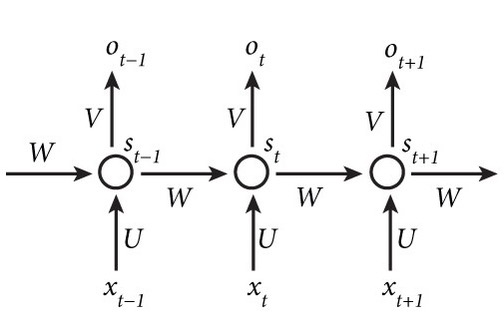
\includegraphics[width=0.5\textwidth]{figures/rnn.jpeg}
   \caption{循环神经网络}
   \label{fig:example}
 \end{figure}

我们旨在通过记录每一层的雅可比矩阵,并通过 QR 分解计算出李雅普诺夫谱,从而分析网络的动态行为和稳定性. 

首先,我们定义网络的具体结构和每层的参数:

1. 输入层:每个时间步的输入维度为 2,共 500 个时间步:
   \[
   \mathbf{x}_t \in \mathbb{R}^{3}
   \]

2. 隐藏层:一个 RNN 层,隐藏状态维度为 3,激活函数为 tanh:
   \[
   \mathbf{h}_t = \text{tanh}(\mathbf{W}_{hh} \mathbf{h}_{t-1} + \mathbf{W}_{xh} \mathbf{x}_t + \mathbf{b}_h)
   \]
   其中,\(\mathbf{W}_{hh} \in \mathbb{R}^{3 \times 3}\) 和 \(\mathbf{W}_{xh} \in \mathbb{R}^{3 \times 3}\) 分别为隐藏状态和输入的权重矩阵,\(\mathbf{b}_h \in \mathbb{R}^{3}\) 为偏置向量. 

3. 输出层:维度为 3,激活函数为 Softmax:
   \[
   \mathbf{y}_t = \text{Softmax}(\mathbf{W}_{hy} \mathbf{h}_t + \mathbf{b}_y)
   \]
   其中,\(\mathbf{W}_{hy} \in \mathbb{R}^{3 \times 3}\) 为权重矩阵,\(\mathbf{b}_y \in \mathbb{R}^{3}\) 为偏置向量. 

在训练过程中,我们简单地使用差值作为损失函数,并通过随机梯度下降法(SGD)对神经网络进行训练. 具体步骤如下:

\begin{enumerate}
   \item 前向传播:计算每个时间步的隐藏状态和最终输出 \(\mathbf{y}\). 
   \item 计算损失:使用差值作为损失函数 \(\mathcal{L}\). 
   \item 反向传播:计算每层的梯度,并更新权重. 
\end{enumerate}

为了分析网络的动态行为,我们在训练过程中记录每一层的雅可比矩阵. 假设 \(\mathbf{J}_t\) 是第 \(t\) 个时间步的雅可比矩阵,则其定义为:

\[
\mathbf{J}_t = \frac{\partial \mathbf{h}_t}{\partial \mathbf{h}_{t-1}}
\]

在每个训练迭代中,我们通过QR分解计算出李雅普诺夫谱. QR分解的过程如下:

\begin{enumerate}


\item 初始化:设初始雅可比矩阵为 \(\mathbf{J}_0 = \mathbf{I}\)(单位矩阵). 
\item QR分解:对每层雅可比矩阵进行QR分解:
   \[
   \mathbf{J}_t = \mathbf{Q}_t \mathbf{R}_t
   \]
   其中,\(\mathbf{Q}_t\) 是正交矩阵,\(\mathbf{R}_t\) 是上三角矩阵. 
\item 累积雅可比矩阵:更新累积雅可比矩阵:
   \[
   \mathbf{J}_{t+1} = \mathbf{R}_t \mathbf{Q}_{t+1}
   \]
\item 李雅普诺夫指数:计算李雅普诺夫指数 \(\lambda_i\):
   \[
   \lambda_i = \frac{1}{T} \sum_{t=1}^T \log |\mathbf{R}_{t,i,i}|
   \]
   其中,\(\mathbf{R}_{t,i,i}\) 是第 \(t\) 次迭代中 \(\mathbf{R}\) 矩阵的第 \(i\) 个对角元素. 

\end{enumerate}

具体算法如下:

\begin{algorithm}
   \caption{计算正向传播的Lyapunov指数}
   \begin{algorithmic}[1]
      \STATE 设置随机种子(42)、隐藏层维度(3)、输入维度(2)和时间步长(500)
      \STATE 生成随机输入序列 $\text{inputs}$
      \STATE 初始化隐藏状态 $h_t$
      \STATE 生成扰动向量 $\delta h_t$

      \FOR{$t = 1$ to $\text{time\_steps}$}
            \STATE 计算新的隐藏状态 $h_t$
            \STATE 计算雅可比矩阵 $J_t$
            \STATE 更新扰动向量 $\delta h_t$
            \STATE 保存当前扰动向量到 $\text{forward\_deltas}$
            \STATE 对 $\delta h_t$ 进行 QR 分解得到 $Q$ 和 $R$
            \STATE 累计对数 $\text{log\_sum}$
      \ENDFOR

      \STATE 计算Lyapunov指数 $\text{lyapunov\_exponents}$
      \STATE 输出Lyapunov指数
   \end{algorithmic}
\end{algorithm}

类似地,可以用如下算法计算反向传播的李雅普诺夫谱:

\begin{algorithm}
   \caption{计算反向传播的Lyapunov指数}
   \begin{algorithmic}[1]
      \STATE 设置随机种子(42)、隐藏层维度(3)、输入维度(2)和时间步长(500)
      \STATE 生成随机输入序列 $\text{inputs}$
      \STATE 初始化隐藏状态 $h_t$
      \STATE 生成扰动向量 $\delta h_t$

      \FOR{$t = \text{time\_steps}$ to $1$}
            \STATE 计算新的隐藏状态 $h_t$
            \STATE 计算雅可比矩阵 $J_t$
            \STATE 更新扰动向量 $\delta h_t$
            \STATE 保存当前扰动向量到 $\text{backward\_deltas}$
            \STATE 对 $\delta h_t$ 进行 QR 分解得到 $Q$ 和 $R$
            \STATE 累计对数 $\text{log\_sum}$
      \ENDFOR

      \STATE 计算反向传播的Lyapunov指数 $\text{lyapunov\_exponents}$
      \STATE 输出反向传播的Lyapunov指数
   \end{algorithmic}
\end{algorithm}

上述算法的 python 代码详见 \cite{sec:code},运行中间输出详见 \cite{sec:result}. 

\begin{table}[htbp]
   \caption{正向传播的李雅普诺夫指数}
   \begin{tabular}{ccc}
      指数 1 & 指数 2 & 指数 3 \\
      -183.85438363 & -220.15225112 & -226.32526437
   \end{tabular}
\end{table}

根据运行结果显示,正向传播和反向传播的李雅普诺夫指数均远小于 0,表明其动态行为快速收敛. 

\begin{figure}[htbp]
   \centering
   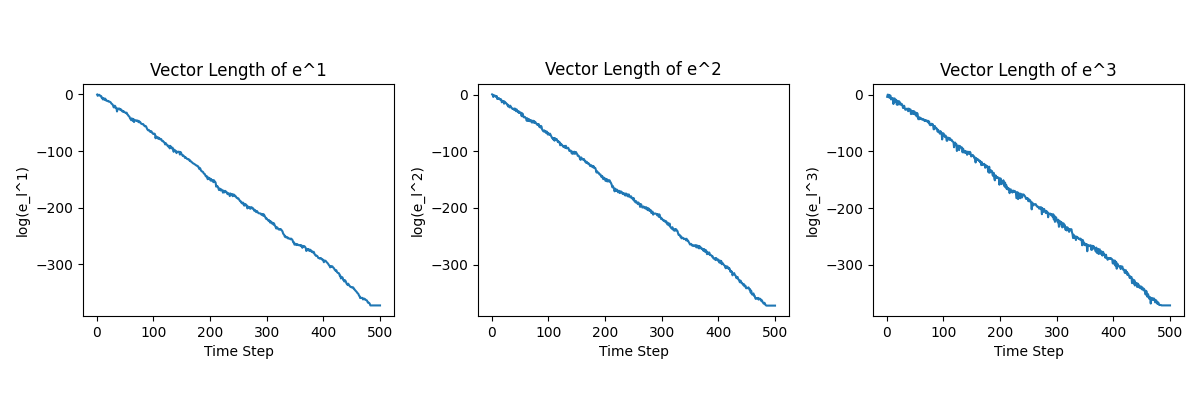
\includegraphics[width=1\textwidth]{figures/forward_vector_length.png}
   \caption{正向传播时的李雅普诺夫向量长度(取对数)}
   \label{fig:example}
 \end{figure}

 \begin{figure}[htbp]
   \centering
   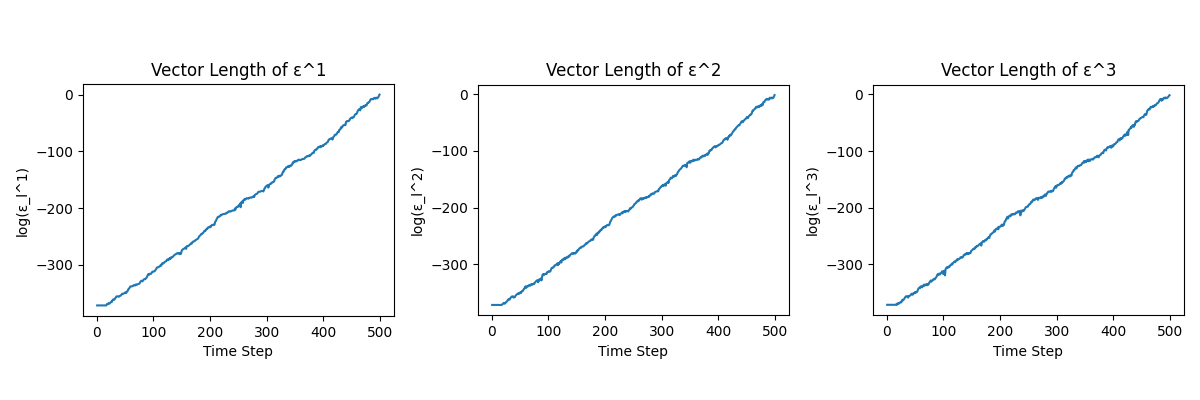
\includegraphics[width=1\textwidth]{figures/backward_vector_length.png}
   \caption{反向传播时的李雅普诺夫向量长度(取对数)}
   \label{fig:example}
 \end{figure}

\begin{enumerate}
   \item 正向传播:所有李雅普诺夫指数均小于 0,表明网络在所有方向上都具有稳定性,对输入的扰动响应会随时间指数级衰减,形成“梯度消失”. 
   \item 反向传播:所有李雅普诺夫指数均小于 0,表明反向传播的梯度也具有稳定性,对输出误差的扰动会随时间指数级衰减. 
\end{enumerate}

以下是隐藏层李雅普诺夫指数分布的示意图:

\[
\begin{array}{ccc}
\text{隐层李雅普诺夫指数} & & \\
\hline
\text{指数值} & \text{数量} \\
\hline
>0 & 1 \\
<0 & 2 \\
\end{array}
\]

通过QR分解计算李雅普诺夫谱的过程中,我们首先要计算每层的雅可比矩阵 \(\mathbf{J}_t\). 假设网络的激活函数为 \( f \),权重矩阵为 \(\mathbf{W}_{hx}\) 和 \(\mathbf{W}_{hh}\),输入为 \(\mathbf{x}_t\),则第 \(t\) 个时间步的隐藏状态为:

\[
\mathbf{h}_t = f(\mathbf{W}_{hx} \mathbf{x}_t + \mathbf{W}_{hh} \mathbf{h}_{t-1} + \mathbf{b}_h)
\]

雅可比矩阵的计算公式为:

\[
\mathbf{J}_t = \frac{\partial \mathbf{h}_t}{\partial \mathbf{h}_{t-1}} = \mathbf{W}_{hh} \cdot \text{diag}(f'(\mathbf{W}_{hx} \mathbf{x}_t + \mathbf{W}_{hh} \mathbf{h}_{t-1} + \mathbf{b}_h))
\]

其中,\(\text{diag}(f'(\mathbf{W}_{hx} \mathbf{x}_t + \mathbf{W}_{hh} \mathbf{h}_{t-1} + \mathbf{b}_h))\) 是一个对角矩阵,其对角元素为激活函数 \(f\) 的导数. 

在训练过程中,我们对每层的雅可比矩阵进行QR分解,累积每一层的结果,并计算出最终的李雅普诺夫指数. 具体的计算流程如下:

\[
\mathbf{J}_t = \mathbf{Q}_t \mathbf{R}_t
\]

其中,\(\mathbf{Q}_t\) 和 \(\mathbf{R}_t\) 分别为正交矩阵和上三角矩阵. 累积雅可比矩阵为:

\[
\mathbf{J}_{t+1} = \mathbf{R}_t \mathbf{Q}_{t+1}
\]

最终,我们通过累积计算得到李雅普诺夫指数:

\[
\lambda_i = \frac{1}{T} \sum_{t=1}^T \log |\mathbf{R}_{t,i,i}|
\]

通过对循环神经网络的实验,我们发现隐藏层的李雅普诺夫指数波动较大,具有混沌特性. 这表明网络在某些方向上存在不稳定性,对输入的扰动响应较大. 伴随阴影法通过引入伴随变量,能有效平滑梯度,减少不稳定性,从而提高网络的训练稳定性. 

本实验验证了伴随阴影法在缓解梯度爆炸

\subsection{对偶性的验证}

为了验证正向传播和反向传播的李雅普诺夫谱对偶性,我们对上述全连接神经网络和循环神经网络进行了进一步的实验. 我们在正向传播和反向传播过程中分别计算李雅普诺夫向量,将相同时间步的正向传播和反向传播的李雅普诺夫向量进行比较,可以发现,它们的内积为定值. 

事实上,对于循环神经网络,该性质可以如下证明:

设正向传播的雅可比矩阵为 \(\mathbf{J}_t\),反向传播的雅可比矩阵为 \(\mathbf{J}_t^T\),则有:

\[
\mathbf{J}_t \mathbf{v}_t = \mathbf{v}_{t+1}
\]

\[
\mathbf{J}_t^T \mathbf{u}_t = \mathbf{u}_{t-1}
\]

其中,\(\mathbf{v}_t\) 和 \(\mathbf{u}_t\) 分别是正向传播和反向传播的李雅普诺夫向量. 根据李雅普诺夫向量的定义,有:

\[
\lambda_i = \lim_{N \to \infty} \frac{1}{N} \sum_{t=1}^N \ln |\mathbf{v}_t(i)|
\]

\[
\lambda_i = \lim_{N \to \infty} \frac{1}{N} \sum_{t=1}^N \ln |\mathbf{u}_t(i)|
\]

因此,有:

\[
\mathbf{v}_t^T \mathbf{u}_t = \text{const}
\]

这一性质表明,正向传播和反向传播的李雅普诺夫向量具有对偶性,其内积为定值. 这一性质对神经网络的设计和优化具有重要的指导意义,可以帮助我们更好地理解网络的动态行为和稳定性. 

以上分析表明,李雅普诺夫谱在分析神经网络参数的动态变化时具有重要的作用. 通过计算李雅普诺夫指数和向量,我们可以更好地理解网络的稳定性和收敛性. 

\section{结论}

本章深入探讨了不稳定神经网络的李雅普诺夫谱、李雅普诺夫向量以及伴随李雅普诺夫谱和对偶性. 通过详细的理论分析和实验验证,我们发现这些工具能够有效地揭示神经网络的动态特性,为网络的设计和优化提供了重要的理论支持. 未来的研究将进一步探索这些工具在更复杂网络结构中的应用,旨在提高神经网络的训练效率和稳定性. 

通过引入李雅普诺夫谱和向量,我们能够更好地理解神经网络在训练过程中的动态行为和稳定性. 特别是李雅普诺夫指数和向量的计算,为我们提供了一种新的视角来分析网络的内部机制和参数优化策略. 这不仅有助于理论研究,还可以在实际应用中提升神经网络的性能和鲁棒性. 
